\section{Spracherweiterungen}

Kurze Beschreibung der Erweiterungen der Sprache. Grundsatz: Kompatibilität beibehalten!

\subsection{Pre-/Postconditions}
Funktionen/Prozeduren mit Pre und Postconditions versehen können.

\subsection{Pure Operationen}
Funktionen/Prozeduren als pur kenzeichnen. -- keine Veränderung von State erlaubt. Dürfen in conditions verwendet werden

%\newpage

%\begin{figure*}[h]
%	\begin{center}
%		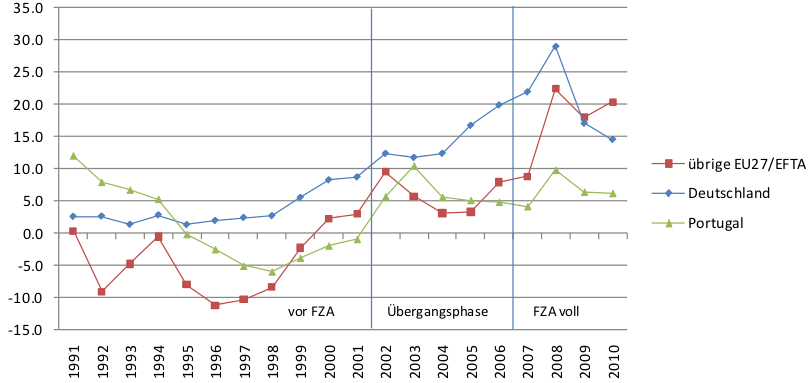
\includegraphics[width=0.9\textwidth]{images/Zuwanderungssaldo_Bericht_2.png}
%	\end{center}
%	\caption{Verlauf der Zuwanderung nach Herkunftsländern in Tausend \cite[S. 18]{ADMIN:Bericht}}
%	\label{fig:zuwanderungsaldi}
%\end{figure*}

